\subsection{Completitud}
Para poder demostrar la completitud debemos considerar árboles infinitos. ¿Qué es un árbol infinito?
\paragraph{}
\begin{definition}
Un árbol se puede ver como un grafo no dirigido $T=\langle N, \, E \rangle$ donde el conjunto $N$ esta formado por los nodos y el conjunto $E$ por las aristas. Un árbol es un \textbf{grafo conexo  acíclico} (entre cada para de nodos hay una sola secuencia de aristas que los unen. Si a un árbol se le quita una arista dejada de ser un grafo conexo. 
\end{definition}
En un árbol finito se verifica la propiedad $\vert \bar{\tau} \vert = \vert N \vert -1 $ como un si y sólo si. 

\begin{definition}
Dados 2 árboles $\arbol{1}$ y $\arbol{2}$, diremos que $T_1$ está incluido en $T_2$ y escribimos $T_1 \leq T_2$ si 
\begin{itemize}
	\item $N_1 \subseteq N_2$ y la raíz coincide
	\item $E_1 \subseteq E_2$
\end{itemize}
\end{definition}
%\paragraph{}
\begin{definition}
Dada una secuencia de árboles 
\[ T_0 \leq T_1 \leq \ldots \leq T_k \leq T_{k+1} \leq \ldots \]
definimos
\end{definition}
\[ \lim_{n \in \mathbb{N}} T_n = \langle N,E \rangle, \mbox{ donde } N= \bigcup_{n\in \mathbb{N}} N_n \mbox{ y } E= \bigcup_{n\in \mathbb{N}} E_n  \]
y la raíz, es la raíz de $T_0$.
\begin{prop} Si $T_0 \leq T_1 \leq \ldots \leq T_k \leq T_{k+1} \leq \ldots$ es una secuencia de árbol. Sea $T= \lim_{n \in \mathbb{N}} T_n$, entonces 
\begin{itemize}
	\item[(a)] $T_i \leq T$ para $i \in \mathbb{N}$
	\item[(b)] $T$ es un árbol
\end{itemize}
\end{prop}
\begin{proof}
La afirmación (a) de la proposición es consecuencia directa de las definiciones. Hay que demostrar que $T$ es conexo. En efecto, tomemos $n_1, \, n_2 \in N$ (nodos de $T$). Puesto que los nodos de $T$ es la unión de todos los nodos y $N_i \subseteq N_j$ para $j>i$. Debe existir $k$ tal que $n_1, \, n_2 \in N_k$. Puesto que $N_k$ es conexo, debe existir una secuencia de aristas $e_1, \ldots, e_l \in E_k$ que unen $n_1$ y $n_2$. Puesto que $E_k \leq \bigcup_{i \in \mathbb{N}}E_i=E$, $e_1, \ldots, e_l \in E$ y por tanto $n_1$ y $n_2$ están conectados en $T$.

Supongamos que existen 2 nodos $n_1$ y $n_2$ de forma que hay 2 caminos $e'_1, \ldots, e'_k$ y $e''_1, \ldots, e''_l$ diferentes que los conectan. De existir $i \in N$ tal que $n_1, \, n_2 \in N_i$ de forma que hay 2 caminos $e'_1, \ldots, e'_k, \, e''_1, \ldots, e''_l \in E_i$. Por tanto en $T_i$ habría 2 formas de conectar $n_1$ y $n_2$. Lo que contradice el hecho de que $T_i$ es un árbol. 
\end{proof}
\paragraph{}
Las reglas de construcción de Tableaux solo extienden ramas abiertas. Es absurdo expandir una rama cerrada. Por tanto si una rama está cerrada, tiene profundidad finita. 
\begin{prop}Si $T$ es un tableau cerrado entonces es finito. 
\end{prop}
\begin{proof}

En primer lugar observemos que en un tableau, el número máximo de descendientes es 2 (cada nodo tiene como mucho 2 hijos correspondientes a la aplicación de una regla de tipo $\beta$). 
\paragraph{}
\begin{minipage}{16cm}
En toda rama hay 2 nodos $n_1$ y $n_2$ que se contradicen
\begin{wrapfigure}{r}{0.25\textwidth} 
    \centering
    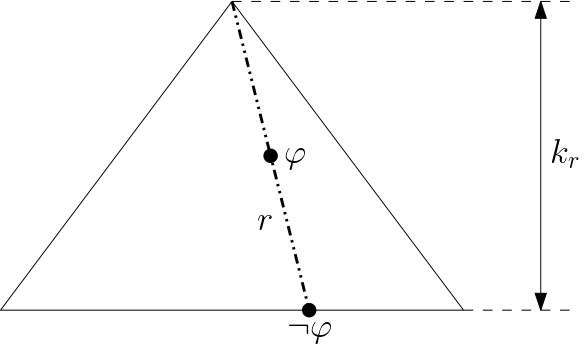
\includegraphics[width=0.25\textwidth]{demo_prop10.png}
\end{wrapfigure}
$h_r= \max \{ \mbox{altura}n_1, \, \mbox{altura}n_2 \}$. Tomamos 
\[ h=\max \{ h_r / r \mbox{ rama de T} \} \]
\begin{itemize}
	\item Si $h < \infty$ como cada nodo tiene como mucho 2 descendientes el árbol es finito. 
	\item Si $h= \infty$ el árbol ha de tener ramas de altura arbitraria. Puesto que cada nodo tiene como mucho 2 descendientes, por el lema de Köning, debe tener una rama infinita. Esa rama infinita no puede estar cerrada puesto que las ramas se cierran siempre a profundidad finita. 
\end{itemize}
\end{minipage}
\end{proof}
\begin{lemma}[\textbf{König}]\cite{hortala_gonzalez_matematica_1998}
Sea $T$ cualquier árbol \textit{localmente finito}, esto es, con la propiedad de que cada nodo interno tiene un número finito de hijos. Si $T$ es infinito, entonces existe en $T$ al menos una rama infinita. 
\end{lemma}
